\section{Results} \label{sec:results}

The benchmarks were run on a machine with the following specifications:
\begin{itemize}
\item Processor: 2 x Intel Xeon E5-2680 v2 @ 3.60GHz (20 Cores / 40 Threads),
MicroArch: IvyBridge
\item OS: Debian 11, kernel: 5.10.0-21-amd64 (x86\_64)
\item Compiler: Clang 15.0.7
\end{itemize}

To gather relevant results, we compiled the whole benchmark suite presented in
Table~\ref{tab:suite} with a single flag presented in Section~\ref{sec:flags} at
a time. Furhtermore we used as baseline the benchmarks compiled with no flag
presented in Section~\ref{sec:flags}. After this step we used Phoronix to run
the generated binaries for each benchmark.

While running a benchmark, Phoronix tries to reduce the noise as much as
possible by rerunning the benchmark until the deviation between the results
becomes minimal. This helped us because we did not have to do any further
calibration to the results.

After compiling and running the benchmarks with all the configurations, we
started to compare each configuration against the baseline. In this step we
recorded the percentage of positive and negative performance impact relative to
the baseline. To take into account noise in the results, we defined the noise
threshold as -2\% for negative performance impact and +2\% for positive
performance impact.

Plots presenting the performance impact for each flag are presented in
Subsection~\ref{sec:flags-results} from Appendix.

For each flag, in nearly 90\% of the cases, the performance impact is
insignificant, i.e. can be considered noise as it is placed between -2\% and
+2\%. 

\textit{-fwrapv} has the biggest overall negative peformance impact, i.e. 11\%
of the results for \textit{-fwrapv} have negative performance impact. This flag
also exhibits the highest negative performance impact as presented in
Figure~\ref{fig:espeak}. Other benchmarks with negative impact: FFTW - Float +
SSE - Size: 1D FFT Size 256, uvg266 (Video Encoder). Other benchmarks with
positive impact: OpenSSL - RSA4096.

\textit{-fno-strict-aliasing} is the most balanced flag up until this moment.
3\% of the results are positive pefrormance impact and 8.2\% of the are negative
performance impact. The outliers for this flag are also very close to the noise
thresholds.

\textit{-fconstrain-shift-value} has many results in the positive impact area,
i.e. 8.1\%. It also has the biggest overall positive performance impact, i.e.
it increases the performance with 35\% relative to baseline. This outlier
exhibits for the benchmark presented in Figure~\ref{fig:gtkperf}. In this
benchmark, \textit{-fconstrain-bool-value} also presents a considerable positive
performance impact.

\textit{-fno-use-default-alignment} exhibits 2 times more positive performance
impact than negative peformance impact. This result is unexpected because in
theory the behavior that this flag exhibits should decrease the peformance of
memory accesses.

\begin{figure}[H]
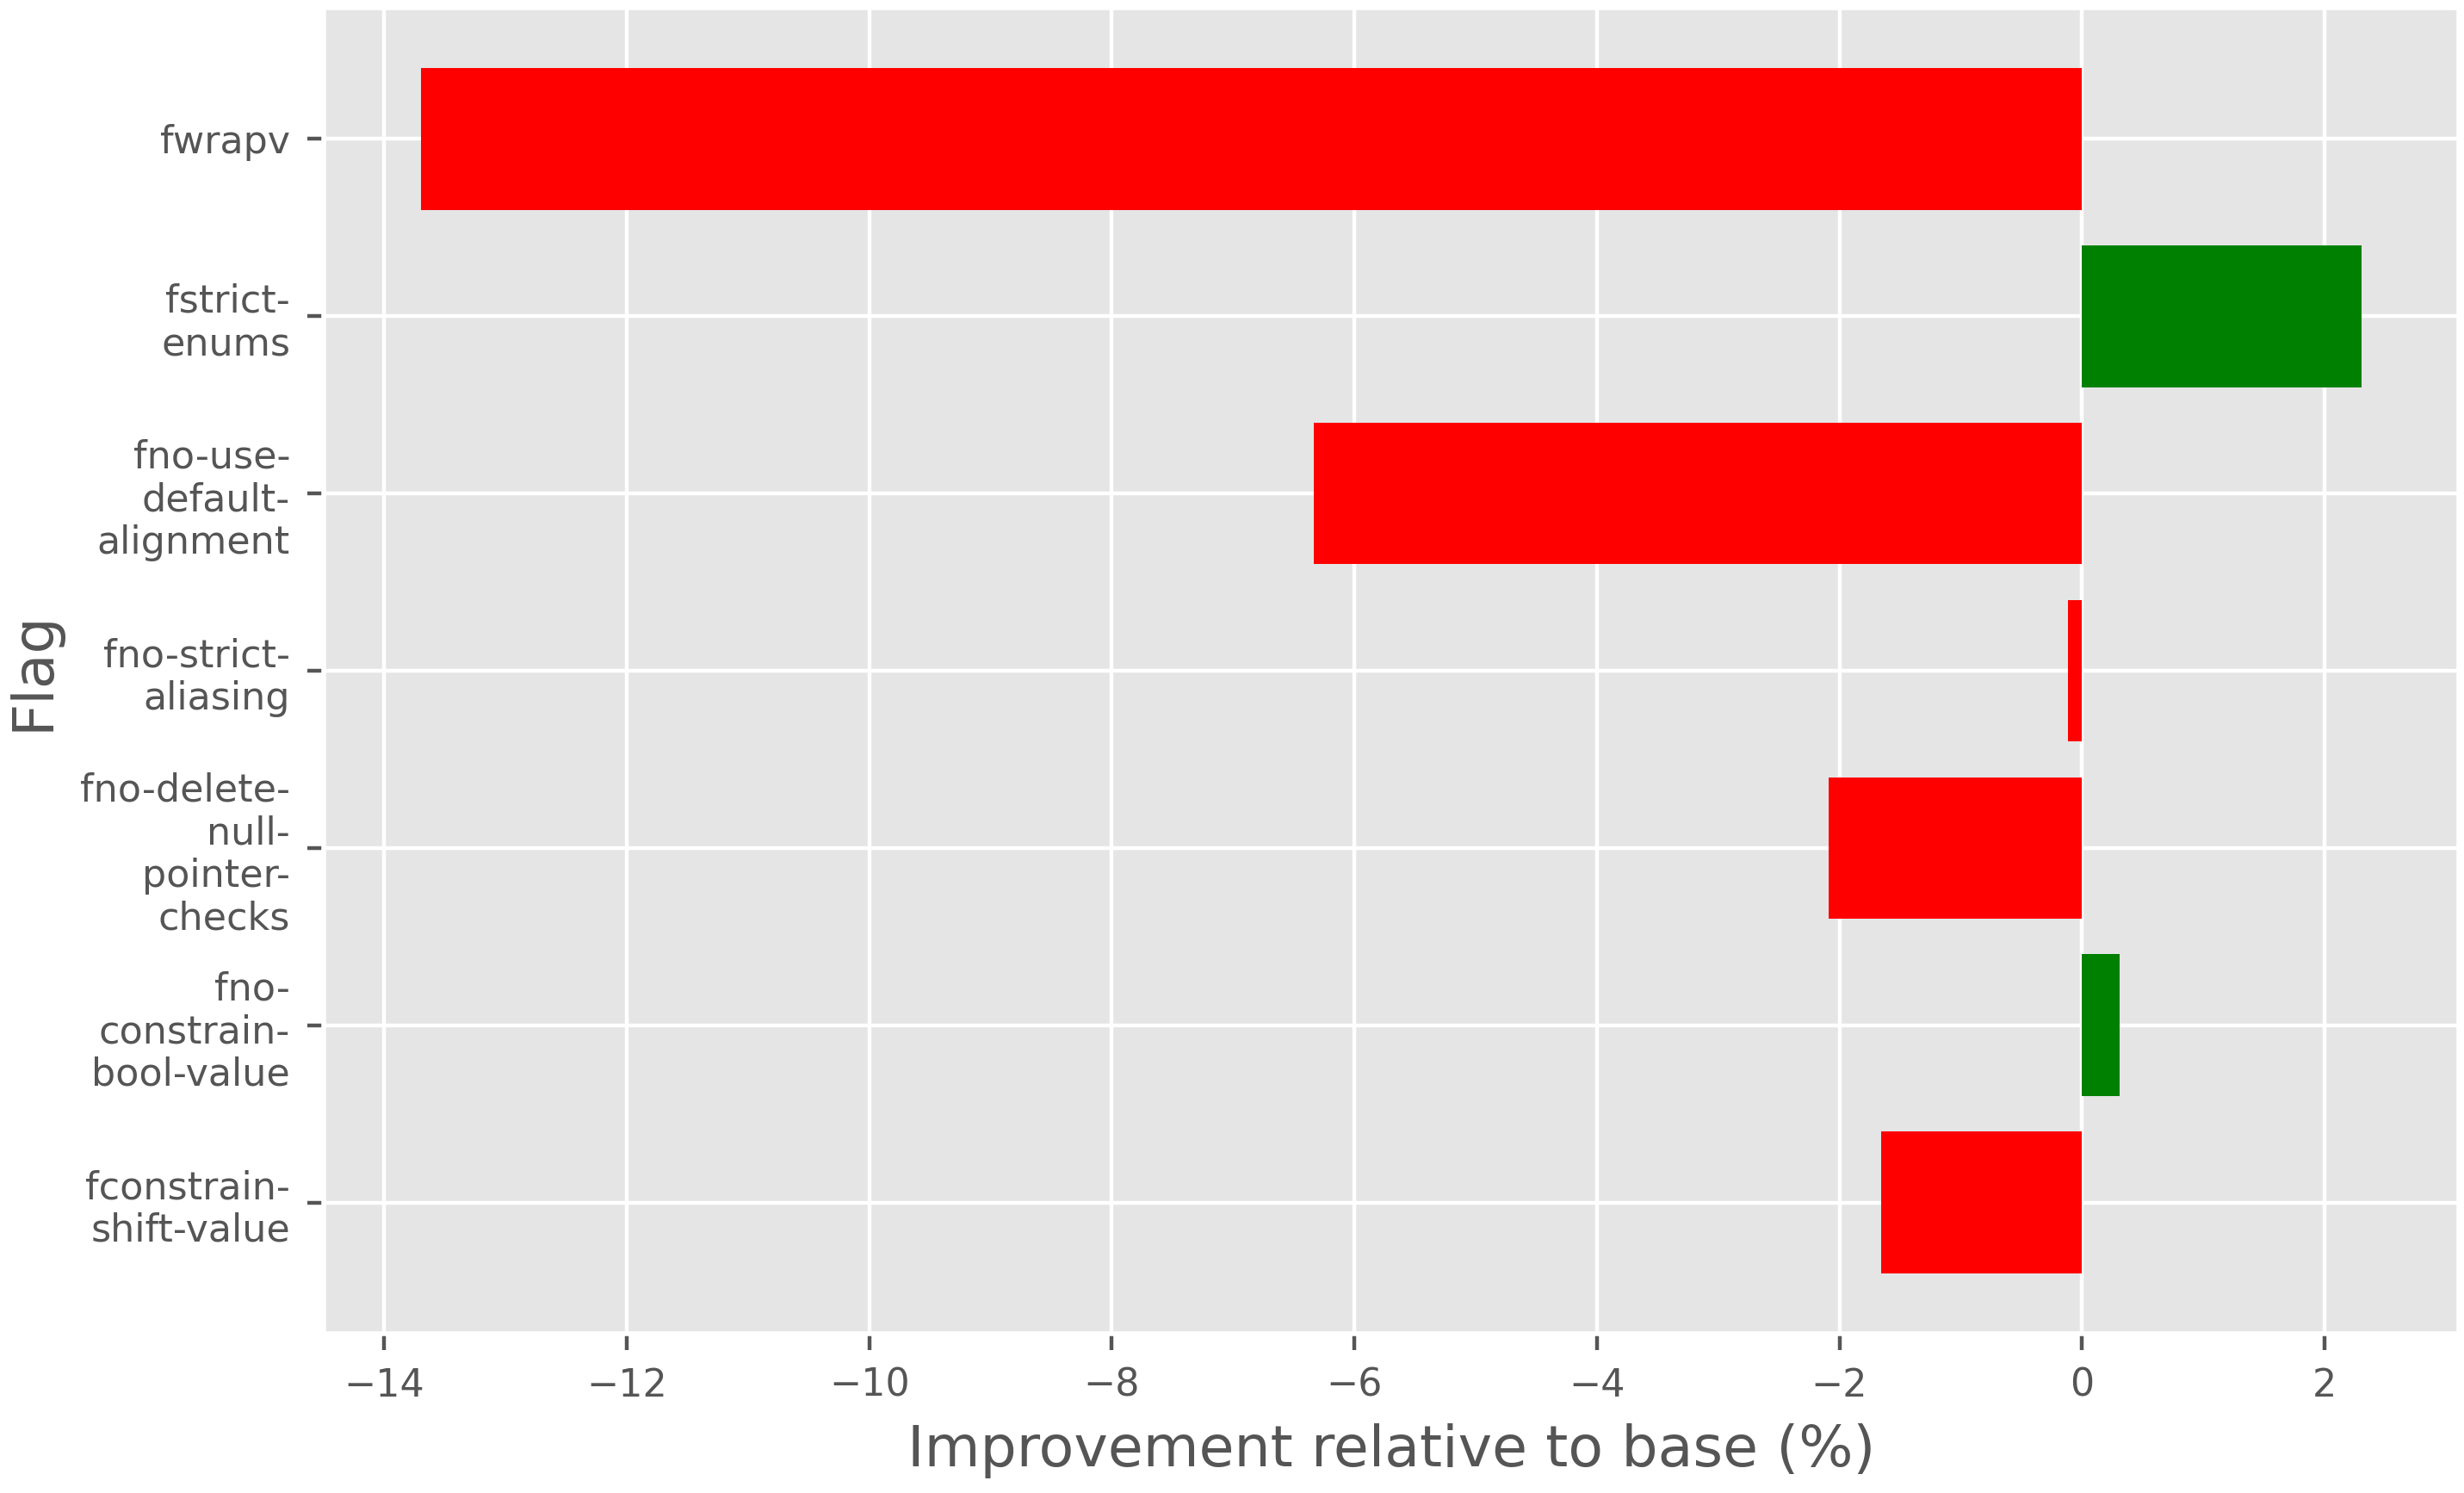
\includegraphics[scale=0.8]{espeak}
\caption{eSpeak-NG Speech Engine - Text-To-Speech Synthesis Benchmark, Baseline:
41.59 Seconds}
\label{fig:espeak}
\end{figure}

\begin{figure}[H]
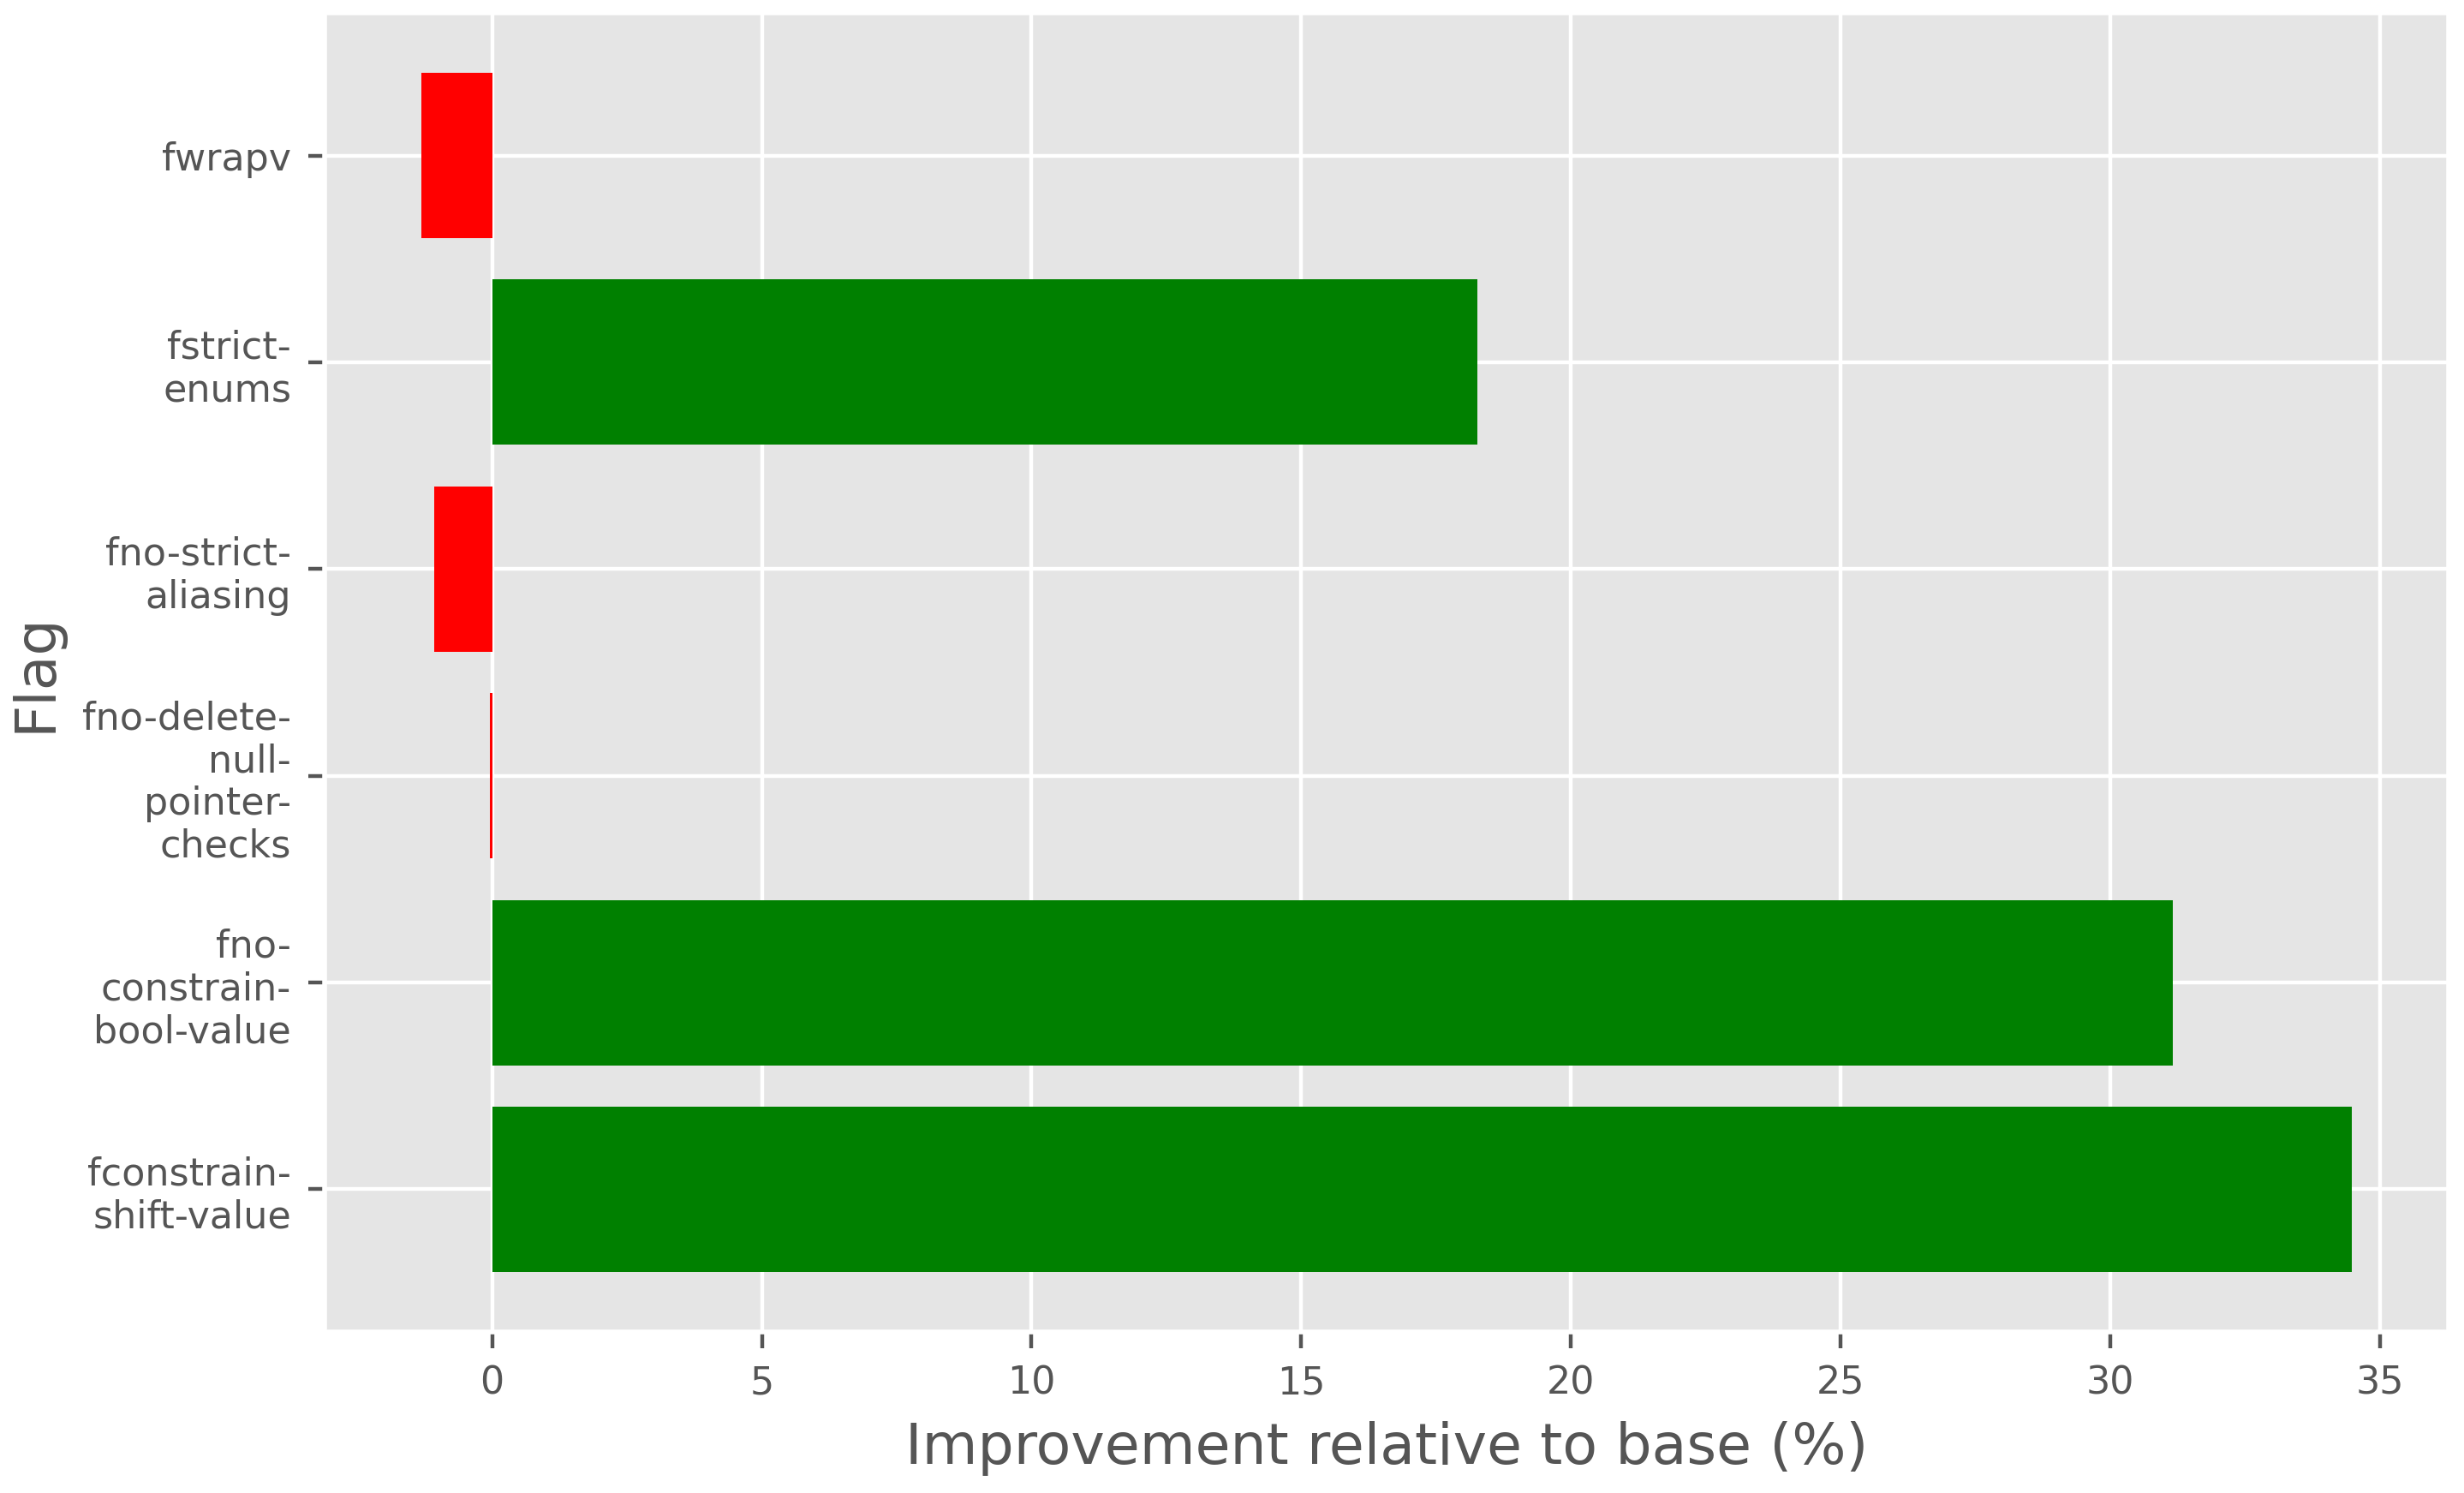
\includegraphics[scale=0.8]{gtkperf}
\caption{GtkPerf - GTK Widget: GtkDrawingArea - PixBufs, Baseline: 170.08
Seconds}
\label{fig:gtkperf}
\end{figure}
